\documentclass[border=4pt,12pt]{standalone}
% House style for redrawn exam diagrams (diagram-v4: 0.4pt lines, filled -latex arrows, fine dashes; stipple and hatching drawn as real dots/lines (no PDF/SVG patterns, so they render in every browser and at any scale); transparent background). Every figure \input's this.
\usepackage{amsmath,amssymb}
\usepackage{txfonts}
\usepackage{pdfrender,xcolor}
% \halo{text}: label on shading. The shading stops just around each letter's outline (a thin knock-out that follows the
% glyphs, like the papers' typesetting), never a box. Owner: "I don't want a box around the text".
\newcommand{\halo}[1]{\leavevmode\rlap{\pdfrender{TextRenderingMode=2,LineWidth=2.2pt,LineJoinStyle=1,StrokeColor=white,FillColor=white}#1}#1}
\usepackage{tikz,pgfplots}
\pgfplotsset{compat=1.18}
\usetikzlibrary{arrows.meta,calc,angles,quotes,patterns,patterns.meta,intersections,positioning,decorations.markings,shapes.geometric}
% Stipple and hatching are drawn as actual dots / lines clipped to the region (path picture), NOT as pattern fills:
% SVG <pattern> fills vanish or blur when browsers scale the image, so the owner could not see the shading.
% Each dot is a 0.72pt square (keeps SVGs small; reads as a dot at print size). Dots sit on one global staggered grid, so neighbouring regions line up.
\makeatletter
\newdimen\ex@x \newdimen\ex@y \newdimen\ex@xa \newdimen\ex@ya \newdimen\ex@xb \newdimen\ex@yb \newcount\ex@row
\def\exam@stipplecolor{black!75}\def\exam@dotr{0.42pt}\def\exam@dotgap{2.5}
\def\ex@rowdots{\ifdim\ex@x<\ex@xb \pgfpathrectangle{\pgfqpoint{\dimexpr\ex@x-0.36pt\relax}{\dimexpr\ex@y-0.36pt\relax}}{\pgfqpoint{0.72pt}{0.72pt}}\advance\ex@x by \exam@dotgap pt\relax\expandafter\ex@rowdots\fi}
\def\exam@stipple{%
  \pgftransformreset% dots are sized in real points even inside scaled pictures
  \pgfpointanchor{path picture bounding box}{south west}\ex@xa=\pgf@x \ex@ya=\pgf@y
  \pgfpointanchor{path picture bounding box}{north east}\ex@xb=\pgf@x \ex@yb=\pgf@y
  \pgfsetfillcolor{\exam@stipplecolor}\pgfmathsetmacro\ex@h{\exam@dotgap/2}%
  \pgfmathtruncatemacro\ex@r{floor(\ex@ya/\ex@h)-1}\ex@row=\ex@r\relax
  \ex@y=\ex@r\dimexpr\ex@h pt\relax
  \loop\ifdim\ex@y<\ex@yb
    \pgfmathtruncatemacro\ex@c{floor(\ex@xa/\exam@dotgap)-1}\ex@x=\ex@c\dimexpr\exam@dotgap pt\relax
    \ifodd\ex@row \advance\ex@x by \ex@h pt\fi
    \ex@rowdots
    \advance\ex@y by \ex@h pt \advance\ex@row by 1
    \ifnum\numexpr\ex@row-(\ex@row/4)*4\relax=0 \pgfusepath{fill}\fi% flush every 4 rows: bounded TeX memory, few clip copies in the SVG
  \repeat\pgfusepath{fill}}
\newdimen\ex@d
\def\exam@hatch#1{% #1 = 1 for /, -1 for \ ; lines 45 degrees, 3pt apart
  \pgftransformreset
  \pgfpointanchor{path picture bounding box}{south west}\ex@xa=\pgf@x \ex@ya=\pgf@y
  \pgfpointanchor{path picture bounding box}{north east}\ex@xb=\pgf@x \ex@yb=\pgf@y
  \ex@d=\dimexpr\ex@yb-\ex@ya\relax \ex@x=\dimexpr\ex@xa-\ex@d\relax
  \loop\ifdim\ex@x<\ex@xb
    \ifnum#1>0 \pgfpathmoveto{\pgfqpoint{\ex@x}{\ex@ya}}\pgfpathlineto{\pgfqpoint{\dimexpr\ex@x+\ex@d\relax}{\ex@yb}}%
    \else \pgfpathmoveto{\pgfqpoint{\ex@x}{\ex@yb}}\pgfpathlineto{\pgfqpoint{\dimexpr\ex@x+\ex@d\relax}{\ex@ya}}\fi
    \advance\ex@x by 4.24pt
  \repeat
  \pgfsetlinewidth{0.4pt}\pgfsetstrokecolor{black}\pgfusepath{stroke}}
\def\examstipple{\exam@stipple}\def\examhatch{\exam@hatch}\def\examsetstipplecolor#1{\def\exam@stipplecolor{#1}}\def\examsetdotgap#1{\def\exam@dotgap{#1}}
\makeatother
% (legacy pattern kept for old files)
% staggered stipple like the NESA papers' dotted shading
\pgfdeclarepatternformonly{exam stipple}{\pgfpointorigin}{\pgfqpoint{2.2pt}{2.2pt}}{\pgfqpoint{2.2pt}{2.2pt}}{%
  \pgfpathcircle{\pgfqpoint{0.55pt}{0.55pt}}{0.42pt}\pgfpathcircle{\pgfqpoint{1.65pt}{1.65pt}}{0.42pt}\pgfusepath{fill}}
\tikzset{
  every picture/.style={line width=0.6pt, >={Latex[length=2mm,width=1.3mm]}},
  curve/.style={line width=0.6pt},
  open arrow/.style={-{Latex[length=2mm,width=1.3mm]}},  % owner: filled -latex heads everywhere, no open chevrons
  aux/.style={dash pattern=on 2pt off 1.5pt, line width=0.6pt},
  shade/.code={\def\exA{#1}\def\exB{none}\ifx\exA\exB\else\pgfkeysalso{fill=black!18}\fi},
  shade/.default=on,
  shade dots/.style={fill=none, path picture={\examstipple}},
  stipple color/.code={\examsetstipplecolor{#1}},
  stipple gap/.code={\examsetdotgap{#1}},
  shade dense dots/.style={fill=none, stipple gap=1.6, path picture={\examstipple}},
  shade hatch/.style={fill=none, path picture={\examhatch{1}}},
  shade hatch reverse/.style={fill=none, path picture={\examhatch{-1}}},
  shade solid/.style={fill=black},
  pt/.style={circle, fill, inner sep=1.1pt},
  open pt/.style={circle, draw, fill=white, inner sep=1.1pt},
}
\pgfplotsset{
  exam axes/.style={axis lines=middle, axis line style={->}, xlabel={$x$}, ylabel={$y$},
    xlabel style={anchor=west}, ylabel style={anchor=south}, tick label style={font=\small},
    every axis plot/.append style={line width=0.6pt, black}, samples=200, clip=false,
    enlargelimits=false, axis on top},
}

\begin{document}
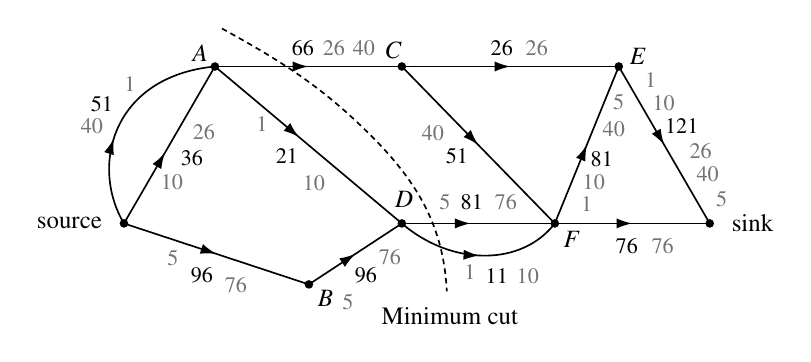
\begin{tikzpicture}[x=0.0127cm,y=-0.0127cm,
  mid/.style={postaction={decorate},decoration={markings,mark=at position #1 with {\arrow{Latex[length=2mm,width=1.3mm]}}}},
  mid/.default=0.5,
  c/.style={font=\footnotesize,inner sep=0.5pt},
  f/.style={font=\footnotesize,inner sep=0.5pt,text=black!55},
  v/.style={font=\small,inner sep=0.5pt},
  dot/.style={circle,fill,inner sep=1.1pt}]
\coordinate (S) at (92,207); \coordinate (A) at (183,50); \coordinate (C) at (370,50);
\coordinate (E) at (587,50); \coordinate (D) at (370,207); \coordinate (F) at (523,207);
\coordinate (T) at (678,207); \coordinate (B) at (277,268);
% edges
\draw[mid=0.4] (S) .. controls (58,150) and (80,60) .. (A);
\draw[mid=0.45] (S) -- (A);
\draw[mid=0.5] (A) -- (C);
\draw[mid=0.5] (C) -- (E);
\draw[mid=0.45] (A) -- (D);
\draw[mid=0.5] (C) -- (F);
\draw[mid=0.5] (F) -- (E);
\draw[mid=0.5] (E) -- (T);
\draw[mid=0.45] (D) -- (F);
\draw[mid=0.5] (F) -- (T);
\draw[mid=0.5] (S) -- (B);
\draw[mid=0.5] (B) -- (D);
\draw[mid=0.5] (D) .. controls (420,250) and (490,250) .. (F);
\foreach \p in {S,A,C,E,D,F,T,B} \node[dot] at (\p) {};
% vertex names
\node[v] at (168,37) {$A$};
\node[v] at (362,34) {$C$};
\node[v] at (606,40) {$E$};
\node[v] at (372,183) {$D$};
\node[v] at (540,223) {$F$};
\node[v] at (293,282) {$B$};
\node[font=\small,anchor=east] at (80,207) {source};
\node[font=\small,anchor=west] at (690,207) {sink};
% source-A (curve)
\node[c] at (70,88) {51}; \node[f] at (98,68) {1}; \node[f] at (60,110) {40};
% source-A (straight)
\node[f] at (172,116) {26}; \node[c] at (160,142) {36}; \node[f] at (140,166) {10};
% A-C
\node[c] at (271,32) {66}; \node[f] at (302,32) {26}; \node[f] at (332,32) {40};
% C-E
\node[c] at (470,32) {26}; \node[f] at (505,32) {26};
% A-D
\node[f] at (230,108) {1}; \node[c] at (255,140) {21}; \node[f] at (282,167) {10};
% C-F
\node[f] at (401,117) {40}; \node[c] at (425,140) {51};
% F-E
\node[f] at (587,86) {5}; \node[f] at (582,113) {40}; \node[c] at (570,143) {81}; \node[f] at (562,166) {10}; \node[f] at (555,188) {1};
% E-sink
\node[f] at (619,64) {1}; \node[f] at (632,87) {10}; \node[c] at (650,110) {121}; \node[f] at (669,135) {26}; \node[f] at (676,158) {40}; \node[f] at (690,183) {5};
% D-F
\node[f] at (413,186) {5}; \node[c] at (440,186) {81}; \node[f] at (474,186) {76};
% F-sink
\node[c] at (595,230) {76}; \node[f] at (631,230) {76};
% S-B
\node[f] at (141,242) {5}; \node[c] at (170,259) {96}; \node[f] at (204,269) {76};
% B-D
\node[c] at (334,259) {96}; \node[f] at (316,286) {5}; \node[f] at (358,241) {76};
% D-F curve
\node[f] at (438,256) {1}; \node[c] at (465,260) {11}; \node[f] at (496,260) {10};
% minimum cut
\draw[aux] (190,12) .. controls (250,45) and (290,70) .. (340,120) .. controls (390,170) and (412,215) .. (415,275);
\node[font=\small] at (418,300) {Minimum cut};
\end{tikzpicture}
\end{document}